% This work is licensed under the Creative Commons
% Attribution-NonCommercial 3.0 Unported License. To view a copy of this
% license, visit http://creativecommons.org/licenses/by-nc/3.0/.

\section{Auswertung}
%
\subsection{Wellenlänge des HeNe-Lasers}
%
Die gemessenen Positionen der n-ten Beugungsmaxima auf dem Schirm 
für die zwei verschiedenen Gitter sind in Tabelle~\ref{tab:welle} 
eingetragen.

Wird von diesen Positionen die Position des nullten Maximums 
abgezogen, ergeben sich die Abstände d der Maxima von der 
optischen Achse. Mit Hilfe von Formel~\eqref{eq:wellenlaenge} 
wird pro Beugungsmaximum eine Wellenlänge berechnet. Dabei 
ist zu beachten, dass der verwendete Schirm bei dem ersten Gitter 
einen Abstand von $L_1 = $ \SI{0.6}{\metre} und der zweite einen 
von $L_2 =$\SI{0.4}{\metre} zum Laser besitzt. 
Das Ergebnis ist ebenfalls in Tabelle~\ref{tab:welle} zu sehen.

%
\begin{table}[h]
  \centering
  \sisetup {
    per-mode = fraction
  }
  \begin{tabular}{SSSS||SSSS}
    \toprule
    \multicolumn{4}{c||}{Gitter mit g = \SI{100}{\per\milli\metre}}&
    \multicolumn{4}{c}{Gitter mit g = \SI{300}{\per\milli\metre}}\\
    {n}&{Pos. /}\si{\centi\metre}&
    {d /}\si{\metre}&$\lambda${ /}\si{\nano\metre}&
    {n}&{Pos. /}\si{\centi\metre}&
    {d /}\si{\metre}&$\lambda${ /}\si{\nano\metre}\\
    \midrule
     -8&2.2&-0.353&633.85&-3&10.2&-0.274&627.92\\
     -7&7.8&-0.297&633.75&-2&21.3&-0.163&628.95\\
     -6&12.8&-0.247&634.45&-1&30.0&-0.076&622.20\\
     -5&17.5&-0.200&632.46&0&37.6&0.000&\% \\
     -4&21.8&-0.157&632.86&1&45.1&0.075&614.30\\
     -3&26.0&-0.115&627.47&2&53.5&0.159&615.65\\
     -2&30.0&-0.075&620.17&3&64.5&0.269&620.05\\
     -1&33.3&-0.042&698.29& &      &        &          \\
      0&37.5&0.000&\%&        &      &        &          \\
      1&41.4&0.039&648.63&   &      &        &          \\
      2&45.2&0.077&636.45&   &      &        &          \\
      3&49.2&0.117&637.98&   &      &        &           \\
      4&53.3&0.158&636.63&   &      &        &           \\
      5&57.5&0.200&632.46&   &      &         &          \\
      6&62.0&0.245&630.05&   &      &        &          \\
      7&66.9&0.294&628.59&   &      &        &          \\
      8&72.5&0.350&620.05&   &      &        &          \\
    \midrule
    \multicolumn{8}{c}{Mittelwerte der Wellenlängen}\\
    \multicolumn{4}{c}{$\lambda_1 = $\SI{637.12(420)}{\nano\metre}}&
    \multicolumn{4}{c}{$\lambda_2 = $\SI{621.51(427)}{\nano\metre}}\\
    \bottomrule
  \end{tabular}
  \caption{Die gemessenen Positisionen der Beugungsmaxima für zwei 
               verschiedene Gitter. Die nullten Beugungsmaxima 
               geben keine Information über die Wellenlänge des 
               Lichtes.}
  \label{tab:welle}
\end{table}
%

\begin{equation}
\lambda = \frac{\sin{\left(\arctan{\left(\frac{d}{L}\right)}\right)}} 
{g\cdot n}
\label{eq:wellenlaenge}
\end{equation}
%

Das arithmetische Mittel der beiden ermittelten Wellenlängenwerte 	
$\lambda_1$ und $\lambda_2$ ergibt als die in diesem Versuch 
bestimmte Wellenlänge des verwendeten Lasers den Wert 
in~\eqref{eq:wellenwert}.
\begin{equation}
\lambda = \frac{\lambda_1 + \lambda_2}{2} = \SI{629.32(420)}{\nano\metre}
\label{eq:wellenwert}
\end{equation}
%
\subsection{Polarisation des HeNe-Lasers}
%

Die Messung des Photostromes in Abhängigkeit des eingestellten 
Polarisationsfilterwinkels ergibt die in 
Tabelle~\ref{tab:polarisation} aufgeführten Messwerte. Daraus liest 
sich der erste maximale Photostrom bei dem Winkel 
$\phi_\text{max} =$ \SI{135}{\degree}. 
%

\begin{table}[h]
  \centering
  \sisetup {
    per-mode = fraction
  }
  \begin{tabular}{SS|SS|SS}
    \toprule
    $\phi${/}\si{\degree}&{Photostrom I/}\si{\milli\ampere}&
    $\phi${/}\si{\degree}&{Photostrom I/}\si{\milli\ampere}&
    $\phi${/}\si{\degree}&{Photostrom I/}\si{\milli\ampere}\\
    \midrule
    0&0.122&125&0.215&245&0.016\\
    5&0.090&130&0.225&250&0.026\\
   10&0.066&135&0.238&255&0.047\\
   15&0.052&140&0.220&260&0.058\\
   20&0.043&145&0.215&265&0.084\\
   25&0.033&150&0.216&270&0.109\\
   30&0.021&155&0.204&275&0.128\\
   35&0.012&160&0.212&280&0.148\\
   40&0.004&165&0.209&285&0.160\\
   45&0.001&170&0.187&290&0.170\\
   50&0.000&175&0.163&295&0.177\\
   55&0.002&180&0.140&300&0.208\\
   60&0.006&185&0.124&305&0.228\\
   65&0.014&190&0.099&310&0.221\\
   70&0.023&195&0.076&315&0.210\\
   75&0.038&200&0.058&320&0.218\\
   80&0.053&205&0.044&325&0.228\\
   85&0.072&210&0.026&330&0.224\\
   90&0.094&215&0.014&335&0.197\\
   95&0.108&220&0.005&340&0.175\\
  100&0.114&225&0.001&345&0.165\\
  105&0.134&230&0.000&350&0.154\\
  110&0.153&235&0.002&355&0.135\\
  115&0.190&240&0.008&360&0.128\\
  120&0.210&     &        &     &       \\
    \bottomrule
  \end{tabular}
  \caption{Die Aufgenommenen Photoströme I in Abhängigkeit des 
               eingestellten Polarisationsfilterwinkels $\phi$.}
  \label{tab:polarisation}
\end{table}
%

Eine Bessere Methode der Bestimmung der Polarisationsrichtung des 
verwendeten Laserlichtes besteht darin, die 
Funktion~\eqref{eq:polarisation} durch die Messwerte zu fitten. Der 
in dieser Formel angegebene Winkel $\delta$ entspricht dann dem 
Polarisationswinkel des Laserlichtes.

%
\begin{equation}
I(\phi) = I_0 \cdot \cos{^2(\phi - \delta)}
\label{eq:polarisation}
\end{equation} 
%

Das Ergebnis dieses Fits\footnote{Zum Fitten der 
Messwerte wird die Funktion \texttt{scipy.optimize.curve\_fit} 
aus der Bibliothek \texttt{scipy-0.10.1} verwendet}, 
sowie ein Plot der Messwerte ist in Abb.~\ref{fig:polarisation} 
zu sehen. Die Fitfunktion ergibt für den Polarisationswinkel 
den Wert
\begin{equation}
\phi_\text{fit} = \SI{139.1(1)}{\degree}.
\end{equation}

%
\begin{figure}
\centering
  \includegraphics[width=0.8\textwidth]{polarisation.pdf}
  \caption{Die gemessenen Photoströme für verschiedene 
Polarisationsfilterwinkel, sowie das Ergebnis des Fits.}
\label{fig:polarisation}
\end{figure}
%
\subsection{Verschiedene TEM-Moden}
%
\paragraph{$\text{TEM}_{000}$ Grundmode}

Die bei dieser Messung erhaltenen Werte für die Photoströme 
für verschiedene Positionen der Photodiode sind in 
Tabelle~\ref{tab:mode1} eingetragen. 
Durch diese wird ein Fit mittels der Gaussfunktion~\eqref{eq:gauss} 
gelegt, wobei r den Abstand zur optischen Achse, w der Strahlradius 
und v der Abstand der Nullposition der verwendeten Photodiode von 
der optischen Achse ist.

Nach Abzug von v von den Photodiodenpositionen ergeben sich 
die Photoströme in Abhängigkeit vom Abstand der Diode zur 
optischen Achse. Diese umgerechneten Werte sind ebenfalls 
in Tabelle~\ref{tab:mode1} eingetragen, sowie in dem 
Plot~\ref{fig:mode1} 
der Messwerte und des Fits als x-Achse verwendet worden.

\begin{equation}
I(r) = I_0 \cdot \exp{\left(-\frac{2(r-v)^2}{w^2}\right)}
\label{eq:gauss}
\end{equation}

%
\begin{table}[h]
  \centering
  \sisetup {
    per-mode = fraction
  }
  \begin{tabular}{SSS}
    \toprule
    {Pos./}\si{\milli\metre}&
    {Photostrom I/}\si{\micro\ampere}&
    {r/}\si{\milli\metre}\\
    \midrule
    -5&0.01&-10.37\\
     0&0.02&-5.37\\
     1&0.11&-4.37\\
     2&0.19&-3.37\\
     3&0.45&-2.37\\
     4&0.83&-1.37\\
     5&1.00&-0.37\\
     6&0.82&0.63\\
     7&0.66&1.63\\
     8&0.42&2.63\\
     9&0.26&3.63\\
     10&0.15&4.63\\
     11&0.09&5.63\\
     12&0.04&6.63\\
     13&0.02&7.63\\
     14&0.01&8.63\\
    \bottomrule
  \end{tabular}
  \caption{Gemessener Photostrom bei verschiedenen Positionen 
    der Photodiode für die Vermessung der TEM-Grundmode. 
     Mit r wird der Abstand zur optischen Achse bezeichnet, welcher 
     sich nach dem Fit als Differenz der Position und dem 
     Fitparameter v in~\eqref{eq:gauss}}
  \label{tab:mode1}
\end{table}
%

Die sich durch den Fit ergebende Funktion ist in 
Formel~\eqref{eq:mode1fit} angegeben.
Darin wird der Strahlradius des Laserstrahles zu 
\begin{equation}
w = \SI{4.17(18)}{\milli\metre}
\end{equation}

\begin{equation}
I_\text{fit} = \SI{0.95}{\micro\ampere}\cdot\exp{\left(-\frac{2r^2}{4.17^2}\right)}
\label{eq:mode1fit}
\end{equation}

%
\begin{figure}
\centering
  \includegraphics[width=0.8\textwidth]{mode1.pdf}
  \caption{Aufgenommene Photoströme für verschiedene Abstände 
zur optischen Achse, sowie das Ergebnis eines Fits, für welchen 
eine Gaussfunktione als Fitfunktion verwendet wird.}
\label{fig:mode1}
\end{figure}

\FloatBarrier
%
\paragraph{$\text{TEM}_{010}$ Oberschwingung}

Analog zum Vorgehen im Paragraphen zur Grundmode, 
sind in Tabelle~\ref{tab:mode2} die entsprechenden Größen 
eingetragen. 

%
\begin{table}[h]
  \centering
  \sisetup {
    per-mode = fraction
  }
  \begin{tabular}{SSS}
    \toprule
    {Pos./}\si{\milli\metre}&
    {Photostrom I/}\si{\micro\ampere}&
    {r/}\si{\milli\metre}\\
    \midrule
    0&0&-10.66\\
   1&0.001&-9.66\\
   2&0.005&-8.66\\
   3&0.007&-7.66\\
   4&0.018&-6.66\\
   5&40&-5.66\\
   6&44&-4.66\\
   7&50&-3.66\\
   8&40&-2.66\\
   9&10&-1.66\\
   10&1&-0.66\\
   11&2&0.34\\
   12&8&1.34\\
   13&12&2.34\\
   14&5&3.34\\
   15&9&4.34\\
   16&8&5.34\\
   17&4&6.34\\
   18&1&7.34\\
   19&0&8.34\\
    \bottomrule
  \end{tabular}
  \caption{Gemessener Photostrom bei verschiedenen Positionen 
    der Photodiode für die Vermessung der erstem TEM-Oberschwingung. 
     Mit r wird der Abstand zur optischen Achse bezeichnet, welcher 
     sich nach dem Fit als Differenz der Position und dem 
     lokalen, mittigen Minimum der Funktion~\ref{zweigauss} ergibt.}
  \label{tab:mode2}
\end{table}
%

Die Funtkion, die durch diese Messwerte gefittert wird, ist eine 
punktweise Überlagerung zweier Gaussfunktionen. Die explizite 
Fitfunktion ist in Gleichung~\eqref{eq:zweigauss} angegeben.

\begin{equation}
I(r) = I_1 \cdot \exp{\left(-\frac{2(r-v_1)^2}{w_1^2}\right)}+
         I_2 \cdot \exp{\left(-\frac{2(r-v_2)^2}{w_2^2}\right)}
\label{eq:zweigauss}
\end{equation}
%

Der Fit durch die Messwerte ergibt die Funktion, welche 
in~\eqref{eq:zweigaussfit} angegeben ist. Ein Plot dieser 
Funktion und der Messwerte gegen r, dem Abstand zur 
optischen Achse, ist in Abb.~\ref{fig:mode2} zu sehen.

\begin{equation}
I_\text{fit} = 
\SI{54.13}{\micro\ampere}\cdot 
\exp{\left(-\frac{2(r)^2}{\SI{2.84}{\milli\metre}^2}\right)}+
\SI{9.77}{\micro\ampere}\cdot 
\exp{\left(-\frac{2(r)^2}{\SI{4.04}{\milli\metre}^2}\right)}
\label{eq:zweigaussfit}
\end{equation}

%
\begin{figure}
\centering
  \includegraphics[width=0.8\textwidth]{mode2.pdf}
  \caption{Aufgenommene Photoströme für verschiedene Abstände 
zur optischen Achse, sowie das Ergebnis eines Fits, für welchen 
zwei Überlagerte Gaussfunktionen als Fitfunktion verwendet werden.}
\label{fig:mode2}
\end{figure}
%

\FloatBarrier

\subsection{Überprüfung der Stabilitätsbedingung}
%
Zuletzt wird die Stabilitätsbedingung des Lasers für 
zwei verschiedene Spiegelgeometrien untersucht.
Die beiden Geometrien werden mit a und b bezeichnet, 
wobei in~\eqref{eq:geometriea} 
und~\eqref{eq:geometrieb} die Krümmungsradien der 
in den jeweiligen Geometrien verwendeten Spiegel 
angegebenen sind.

\begin{equation}
r_1 = r_2 = \SI{1.4}{\metre}
\label{eq:geometriea}
\end{equation} 

\begin{equation}
r_1 = \SI{1}{\metre}\text{ ; }r_2=\SI{1.4}{\metre}
\label{eq:geometrieb}
\end{equation}

In Tabelle~\ref{tab:stabil} sind die maximal einstellbaren 
Intensitäten des Laserstrahls für verschiedene Spiegelabstände 
eingetragen. Plot~\ref{fig:stabil} zeigt schematisch den 
Vergleich zwischen experimentell ermittelten Stabilitätsgebieten 
und theoretisch vorhergesagten Stabilitätsgebieten, wobei 
angenommen wird, dass zwischen kleinstem gemessenen 
Spiegelabstand und einem Abstand von Null die 
Stabilitätsbedingung auch experimentell erfüllt ist.

%
\begin{table}[h]
  \centering
  \sisetup {
    per-mode = fraction
  }
  \begin{tabular}{SS||SS}
    \toprule
    \multicolumn{2}{c||}{Spiegelgeometrie a}&
    \multicolumn{2}{c}{Spiegelgeometrie b}\\
    {Abstand L/}\si{\metre}&{Photostrom I/}\si{\milli\ampere}&
    {Abstand L/}\si{\metre}&{Photostrom I/}\si{\milli\ampere}\\
    \midrule
 1.92&0.080&0.61&7.44\\
 1.82&  0.087&0.81&8.73\\
 1.72&  0.110&0.91&8.92\\
 1.62&  0.171&1.01&2.09\\
 1.52&  0.253&1.05&0.18\\
 1.42&  0.400&{Von}1.06{ bis }1.45&0\\
 1.32&  0.360&1.46&0.07\\
 1.22&  0.268&1.56&6.3\\
 1.12&  0.270&1.62&10.3\\
 1.02&  0.450&      &      \\
 0.92&  0.399&      &      \\
 0.82&  0.422&      &      \\
    \bottomrule
  \end{tabular}
  \caption{Die maximal erreichten Photoströme, welche 
proportional zur Laserstrahlintensität sind, für verschiedene 
Spiegelabstände- und geometrien. Es ist zu beachten, dass für 
Anordnung b ein Bereich existiert, in dem die Stabilitätsbedingung 
nicht erfüllt wird, vor und hinter diesem aber schon.}
  \label{tab:stabil}
\end{table}
%

%
\begin{figure}
\centering
  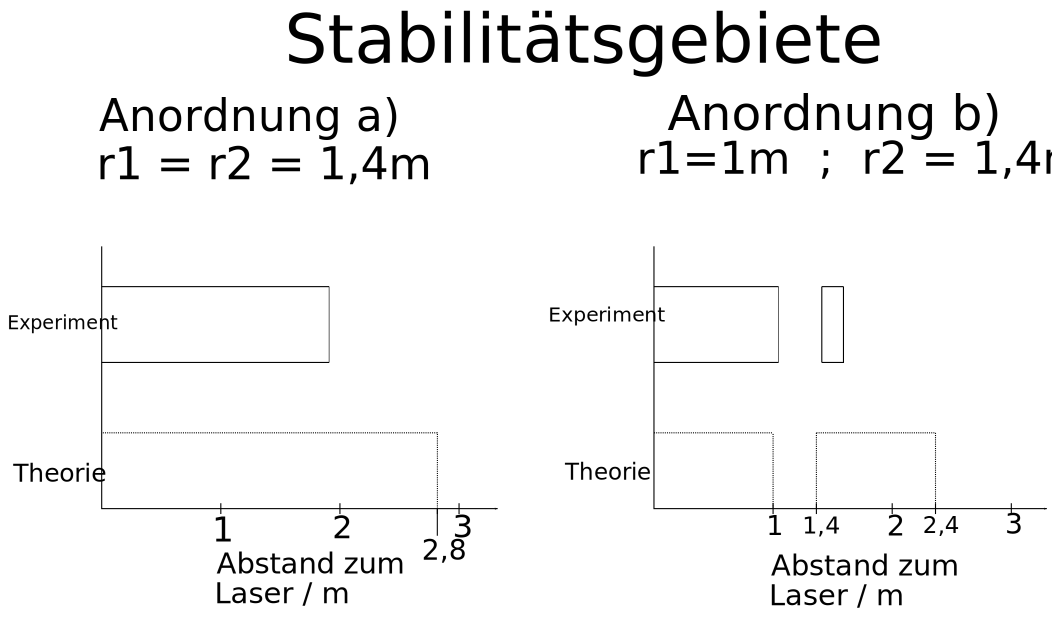
\includegraphics[width=0.8\textwidth]{stabil.pdf}
  \caption{Graphische Darstellung von theoretisch vorhergesagtem 
und experimentell erreichten Stabilitätsgebieten.}
\label{fig:stabil}
\end{figure}
%

%